\documentclass[11pt,a4paper]{article}
\usepackage[margin=1in]{geometry}
\usepackage{booktabs}
\usepackage{array}
\usepackage{multirow}
\usepackage{pgfplots}
\usepackage{siunitx}
\usepackage{enumitem}
\usepackage{hyperref}
\usepackage{longtable}
\pgfplotsset{compat=1.18}
\sisetup{round-mode=places,round-precision=4}

\title{DNN Hyperparameter Tuning Report\\{\large ML vs DNN Comparison across 10 Dashboard Tasks}}
\author{Bellatreche Mohamed Amine}
\date{\today}

\begin{document}
\maketitle
\vspace{-0.8em}

% ──────────────────────────────────────────────────────────────
\section{Introduction}
% ──────────────────────────────────────────────────────────────

After building the ML baselines for our Streamlit dashboard (Stacking classifiers, XGBoost, Ridge, Random Forest, etc.), we wanted to see how a deep neural network would perform on the same tasks using the exact same data and preprocessing.
The idea was not to replace the ML models, but to actually understand where DNNs help and where they don't, especially on our kind of tabular data.

We ran a proper hyperparameter search for each task --- 15 different MLP configurations per task --- varying the network depth, width, activation function, regularisation strength, and learning rate.
All of this was done with \texttt{sklearn.neural\_network.MLPClassifier/MLPRegressor} with early stopping enabled.

\begin{itemize}[leftmargin=1.2em,itemsep=0.2em]
    \item Total tasks benchmarked: \textbf{10}
    \item DNN configurations tested per task: \textbf{15}
    \item DNN wins: \textbf{4} (COVID, Employee anomaly, Heart anomaly, Wine anomaly)
    \item ML wins: \textbf{6}
    \item Preprocessing verified identical to ML: all 10 tasks
\end{itemize}

% ──────────────────────────────────────────────────────────────
\section{Methodology}
% ──────────────────────────────────────────────────────────────

\subsection{Preprocessing Alignment}

Before training any DNN, we made sure the preprocessing was the same as the ML baselines. We checked each task against the saved model metadata JSONs:

\begin{itemize}[leftmargin=1.2em,itemsep=0.15em]
    \item \textbf{Heart:} \texttt{StandardScaler} + stratified split --- same as Stacking ML model.
    \item \textbf{COVID:} \texttt{KNNImputer(k=5)} + \texttt{StandardScaler} + stratified split --- same as ML Stacking (LR meta-learner).
    \item \textbf{Temperature:} Drop 3 columns, NaN-preserving \texttt{LabelEncoder}, \texttt{KNNImputer(k=5)}, \texttt{StandardScaler} --- identical to ML Stacking pipeline.
    \item \textbf{Multi-output:} Drop 2 columns, zero-pressure $\rightarrow$ NaN, NaN-preserving label encode, joint \texttt{KNNImputer(k=5)} on $X+y$ --- same as XGBoost multi-output.
    \item \textbf{Weather:} 31 engineered features (cyclic time, interactions, rolling stats), distribution-based imputation + \texttt{IterativeImputer}, \texttt{StandardScaler} --- matches Random Forest pipeline.
    \item \textbf{Wind \& Energy forecasting:} \texttt{MinMaxScaler} + sliding window (size 24) --- same as Ridge models.
    \item \textbf{Anomaly tasks:} Same train/test splits, label mapping, \texttt{StandardScaler} --- matches Elliptic Envelope / DBSCAN baselines.
\end{itemize}

This way, any difference in score comes from the model itself, not from different data preparation.

\subsection{Hyperparameter Search Setup}

We defined 15 configurations that cover the main axes you would normally tune for an MLP:

\begin{center}
\small
\begin{tabular}{ll}
\toprule
\textbf{Hyperparameter} & \textbf{Values explored} \\
\midrule
Hidden layers & (64), (128), (128,64), (256,128), (128,64,32), (256,128,64) \\
Activation & ReLU, Tanh \\
L2 regularisation ($\alpha$) & 0.0001, 0.001, 0.01 \\
Learning rate init & 0.001, 0.01 \\
\bottomrule
\end{tabular}
\end{center}

All models used \texttt{adam} solver, \texttt{max\_iter=300}, \texttt{early\_stopping=True} with \texttt{n\_iter\_no\_change=5}.
For large datasets ($>$20k rows, like temperature or weather), we subsampled to 20k during the HP search to keep things manageable, then retrained the best config on the full training set.

\subsection{Fallback Mechanism for Weather}

We ran into an issue with weather classification: the best config on the 20k subsample (a large 256$\times$128$\times$64 net with lr=0.01) completely diverged when retrained on the full 70k dataset, giving AUC=0.50 (random).
To handle this, we added a fallback: after the HP search, we rank all configs by their subsample score and try retraining them one by one on the full data.
If the full-retrain score drops more than 10\% compared to the subsample score, we skip it and try the next one.
This way we ended up with MLP(128$\times$64, relu, $\alpha$=0.001, lr=0.001) which gave a stable AUC of 0.6407.

% ──────────────────────────────────────────────────────────────
\section{Final Results: ML vs DNN}
% ──────────────────────────────────────────────────────────────

\small
\begin{tabular}{p{3.1cm} p{1.2cm} p{1.5cm} p{1.5cm} p{1.5cm} p{1.0cm}}
\toprule
\textbf{Task} & \textbf{Metric} & \textbf{ML} & \textbf{DNN} & \textbf{$\Delta$ (DNN-ML)} & \textbf{Winner} \\
\midrule
Heart classification & ROC-AUC & 0.9784 & 0.9416 & $-$0.0368 & ML \\
COVID classification & AUC-ROC & 0.8975 & 0.9009 & +0.0034 & DNN \\
Temperature regression & $R^2$ & 0.7766 & 0.7439 & $-$0.0327 & ML \\
Multi-output regression & Avg $R^2$ & 0.9282 & 0.4665 & $-$0.4617 & ML \\
Weather classification & AUC & 0.8493 & 0.6407 & $-$0.2086 & ML \\
Wind forecasting & $R^2$ & 0.9714 & 0.9706 & $-$0.0008 & ML \\
Energy forecasting & $R^2$ & 0.9985 & 0.9977 & $-$0.0008 & ML \\
Anomaly (Employee) & F1 & 0.4694 & 0.7423 & +0.2729 & DNN \\
Anomaly (Heart) & Bal.\ Acc. & 0.6640 & 0.7711 & +0.1071 & DNN \\
Anomaly (Wine) & F1 & 0.9188 & 0.9937 & +0.0749 & DNN \\
\bottomrule
\end{tabular}

\normalsize
\vspace{0.6em}

% ──────────────────────────────────────────────────────────────
\section{Per-Task Hyperparameter Analysis}
% ──────────────────────────────────────────────────────────────

Here we go through each task, what configs we tried, and what we observed. All 15 configs were evaluated; we report the top-3 and worst to give a sense of the spread.

\subsection{Heart Disease Classification}

\textbf{Best config:} MLP(256$\times$128, relu, $\alpha$=0.0001, lr=0.01) $\rightarrow$ ROC-AUC = 0.9416.

The scores ranged from 0.8898 (single 64-neuron layer) up to 0.9416. The key factor here was the learning rate: bumping lr from 0.001 to 0.01 clearly helped, with the top~3 configs all using lr=0.01. Deeper networks also did better --- (256,128) and (256,128,64) beat the shallower ones. Tanh activation was slightly worse than relu across the board.

Still, the ML Stacking ensemble (0.9784) beats DNN by about 3.7 points. The dataset is relatively small ($\sim$900 samples), which is exactly where ensemble methods tend to have an edge because they combine multiple weak learners that each capture different patterns. The MLP doesn't have that diversity.

\subsection{COVID-19 Classification}

\textbf{Best config:} MLP(128$\times$64, relu, $\alpha$=0.0001, lr=0.01) $\rightarrow$ AUC-ROC = 0.9009.

This is one of the tasks where the DNN actually beats the ML model (Stacking LR, 0.8975), even if the margin is tiny (+0.0034). The top configs here were the ones with lr=0.01 --- MLP(128$\times$64) and MLP(256$\times$128) both hit around 0.900. The worst was the single 64-neuron layer (0.8145). Regularisation didn't matter much; $\alpha$=0.0001 and $\alpha$=0.001 gave nearly the same result at the same architecture.

One thing we noticed is that the dataset has 33 blood markers with quite a bit of missing data (handled by KNNImputer), and the MLP seems to handle the imputed feature space reasonably well. The fact that a simple 2-layer MLP ties or slightly beats a 5-model stacking ensemble is interesting --- it suggests the decision boundary for this problem might be smoother than expected.

\subsection{Temperature Regression}

\textbf{Best config:} MLP(256$\times$128$\times$64, relu, $\alpha$=0.0001, lr=0.001) $\rightarrow$ $R^2$ = 0.7439.

The spread across 15 configs was pretty narrow (0.718 to 0.732 on the subsample). Deeper networks did marginally better, and tanh was about the same as relu. Higher learning rate (0.01) actually hurt slightly here.
After retraining the best config on the full 96k training set, the score went up to 0.7439, but the ML Stacking model still wins (0.7766). The gap ($\sim$3.3 points) makes sense: the temperature dataset has a lot of categorical features and non-linear interactions (weather descriptions, daily summaries) that tree-based models in the stacking ensemble capture better with their built-in feature splits.

\subsection{Multi-Output Regression (Pressure + Humidity)}

\textbf{Best config:} MLP(128$\times$64$\times$32, relu, $\alpha$=0.0001, lr=0.001) $\rightarrow$ Avg $R^2$ = 0.4665.

This is by far the worst DNN result relative to ML. The XGBoost multi-output model gets 0.9282 while the best MLP barely reaches 0.47.
Looking at the per-target breakdown, humidity prediction is okay (best $R^2 \approx 0.655$) but pressure prediction is terrible ($R^2 \approx 0.20$). The tanh configs were even worse for pressure, some going to $R^2 \approx 0$.

We think the problem is that pressure has a very different scale and distribution from humidity, and the \texttt{MultiOutputRegressor} wrapper trains one independent MLP per target. The MLP for pressure struggles to converge because the signal is weaker and the loss landscape is harder. XGBoost on the other hand handles each target's quirks much better through its boosting process.

\subsection{Weather Classification (4-class)}

\textbf{Best stable config:} MLP(128$\times$64, relu, $\alpha$=0.001, lr=0.001) $\rightarrow$ AUC = 0.6407.

This task was tricky. On the 20k subsample, the best score was 0.7097 from MLP(256$\times$128$\times$64, relu, lr=0.01), but when we retrained on the full 70k data, it diverged completely (AUC dropped to 0.50). The higher learning rates (lr=0.01) were unstable on this large dataset, with two of the three lr=0.01 configs on the subsample already scoring below 0.50.

After the fallback mechanism kicked in, we settled on a smaller, more conservative config (lr=0.001, $\alpha$=0.001) that transferred well to the full data. Still, the Random Forest model (0.8493) is way ahead. Weather classification has 4 classes with a lot of overlap between ``Mostly Cloudy'' and ``Overcast,'' and the 31 engineered features were designed around tree-based splits --- the MLP doesn't benefit from them in the same way.

\subsection{Wind Turbine Forecasting}

\textbf{Best config:} MLP(256$\times$128, relu, $\alpha$=0.0001, lr=0.01) $\rightarrow$ $R^2$ = 0.9706.

All 15 configs scored between 0.9698 and 0.9711 --- the spread is really tiny. Basically every architecture we tried works almost equally well. This makes sense because the sliding window approach (size 24) already captures most of the temporal pattern, so even a small network can fit the residuals.

The ML Ridge model (0.9714) is only 0.08 percentage points ahead. Given how close these are, the difference is probably just noise. If we had to pick, we'd say the task is well-suited for both approaches because the feature engineering (the window) does most of the heavy lifting.

\subsection{Energy Consumption Forecasting}

\textbf{Best config:} MLP(256$\times$128, relu, $\alpha$=0.0001, lr=0.001) $\rightarrow$ $R^2$ = 0.9977.

Very similar story to wind. All configs scored between 0.9926 and 0.9962 on the 20k subsample, and the best retrained on the full 116k dataset gave 0.9977. The ML Linear Regression is at 0.9985 --- the difference is less than 0.1\%.

One interesting thing: higher regularisation ($\alpha$=0.01) and higher lr (0.01) both degraded performance slightly, suggesting the problem is very well-conditioned and doesn't need aggressive regularisation. The sliding window does most of the work here too.

\subsection{Anomaly Detection: Employee Attrition}

\textbf{Best config:} MLP(256$\times$128, relu, $\alpha$=0.001, lr=0.001) $\rightarrow$ F1 = 0.7423.

This is where the DNN really shines compared to ML. The ML baseline (DBSCAN, F1=0.4694) was already known to be weak because anomaly detection is being used in an unusual way here --- we're treating attrition as the ``anomaly'' class and using supervised features.
All 15 MLP configs beat the ML baseline, with scores ranging from 0.7156 to 0.7423. Tanh configs were slightly better (top tanh: 0.7397) than default relu configs, probably because the feature interactions for employee behaviour are somewhat non-linear but smooth. The extra regularisation ($\alpha$=0.001 to 0.01) helped a bit compared to $\alpha$=0.0001.

The DNN wins here by a huge margin (+0.273) because it's actually doing supervised classification while the ML model was doing unsupervised anomaly detection --- so the comparison is a bit unfair to the ML side, honestly.

\subsection{Anomaly Detection: Heart Disease}

\textbf{Best config:} MLP(64, relu, $\alpha$=0.0001, lr=0.001) $\rightarrow$ Balanced Accuracy = 0.7711.

This is interesting because the simplest config won. The single 64-neuron layer beats all the deeper architectures. Many of the larger configs (256$\times$128, 128$\times$64$\times$32) collapsed to balanced accuracy = 0.50 --- basically predicting everything as one class.
This is a classic sign of overfitting on a small, imbalanced dataset. The smaller network generalizes better because it can't memorize the training data.

The ML baseline (Elliptic Envelope, 0.6640) is beaten by +10.7 points. Again, the DNN has the advantage of supervised labels while the ML model is doing unsupervised detection.

\subsection{Anomaly Detection: Wine Type}

\textbf{Best config:} MLP(128$\times$64$\times$32, relu, $\alpha$=0.0001, lr=0.001) $\rightarrow$ F1 = 0.9937.

Almost perfect. Most configs scored above 0.977, and even the ``worst'' (256$\times$128 with $\alpha$=0.001) still hit 0.977. The task is structurally easy: red vs white wine from chemical features, with the minority class (red) treated as the anomaly. The chemical signatures are quite distinct, so basically any reasonable classifier will do well. The DNN's 0.9937 beats Elliptic Envelope's 0.9188 by about 7.5 points.

% ──────────────────────────────────────────────────────────────
\section{Visual Summary}
% ──────────────────────────────────────────────────────────────

\begin{center}
\begin{tikzpicture}
\begin{axis}[
    width=0.92\textwidth,
    height=0.32\textheight,
    ybar,
    bar width=5.5pt,
    ylabel={$\Delta$ (DNN $-$ ML)},
    symbolic x coords={Heart,COVID,Temp,MultiOut,Weather,Wind,Energy,EmpAnom,HeartAnom,WineAnom},
    xtick=data,
    x tick label style={rotate=35,anchor=east,font=\scriptsize},
    yticklabel style={font=\scriptsize},
    nodes near coords,
    nodes near coords style={font=\tiny, /pgf/number format/fixed, /pgf/number format/precision=3},
    enlargelimits=0.03,
    grid=major
]
\addplot coordinates {
(Heart,-0.0368)
(COVID,+0.0034)
(Temp,-0.0327)
(MultiOut,-0.4617)
(Weather,-0.2086)
(Wind,-0.0008)
(Energy,-0.0008)
(EmpAnom,+0.2729)
(HeartAnom,+0.1071)
(WineAnom,+0.0749)
};
\end{axis}
\end{tikzpicture}

\vspace{0.4em}
\begin{tikzpicture}
\begin{axis}[
    width=0.52\textwidth,
    height=0.22\textheight,
    ybar,
    bar width=18pt,
    symbolic x coords={DNN Wins,ML Wins},
    xtick=data,
    ylabel={Task count},
    ymin=0,ymax=10,
    nodes near coords,
    nodes near coords style={font=\small},
    grid=major
]
\addplot coordinates {(DNN Wins,4) (ML Wins,6)};
\end{axis}
\end{tikzpicture}
\end{center}

% ──────────────────────────────────────────────────────────────
\section{PyTorch Framework Experiments}
% ──────────────────────────────────────────────────────────────

After running the sklearn MLP hyperparameter search we realised there were things we simply couldn't test:
dropout layers, batch normalisation, proper decoupled weight decay (AdamW), and learning-rate schedulers.
All of these are standard practice in deep learning but aren't exposed by \texttt{sklearn.neural\_network.MLPClassifier/Regressor}.
So we ran a follow-up experiment on two tasks --- heart classification and temperature regression --- using PyTorch directly.

We kept the base architecture identical to the sklearn best (no unfair advantage): 256$\times$128 for heart, 256$\times$128$\times$64 for temperature, ReLU activation, same train/val/test splits, same preprocessing pipelines.
Then we tested 10 configurations, each isolating a specific new capability.

\subsection{PyTorch-Specific Hyperparameters Tested}

\begin{center}
\small
\begin{tabular}{lll}
\toprule
\textbf{Config} & \textbf{What it adds over sklearn baseline} & \textbf{Key parameter} \\
\midrule
\texttt{pt\_baseline}          & Direct replication of sklearn best & Adam, wd=1e-4 \\
\texttt{pt\_dropout\_02}       & Dropout between hidden layers       & $p=0.2$ \\
\texttt{pt\_dropout\_04}       & Heavy dropout                       & $p=0.4$ \\
\texttt{pt\_batchnorm}         & BatchNorm1d after each linear       & no dropout \\
\texttt{pt\_bn\_dropout}       & BN + dropout combined               & BN + $p=0.2$ \\
\texttt{pt\_adamw}             & AdamW (decoupled weight decay)      & wd=0.01 \\
\texttt{pt\_sgd\_momentum}     & SGD with Nesterov momentum          & mom=0.9 \\
\texttt{pt\_scheduler\_plateau}& Adam + \texttt{ReduceLROnPlateau}  & factor=0.5, patience=5 \\
\texttt{pt\_scheduler\_cosine} & Adam + \texttt{CosineAnnealingLR}  & $T_\text{max}$=max\_epochs \\
\texttt{pt\_full\_modern}      & BN + Dropout + AdamW + Cosine       & ``kitchen sink'' \\
\bottomrule
\end{tabular}
\end{center}

Training used early stopping (patience 25 for heart, 10 for temperature) and Kaiming (He) initialisation for all linear layers.
For temperature, we subsampled to 15k rows during the HP search (same strategy as the sklearn experiments) and retrained each config on the full 62k training set.

\subsection{Heart Classification Results}

\begin{center}
\small
\begin{tabular}{lcccc}
\toprule
\textbf{Config} & \textbf{Dropout} & \textbf{BN} & \textbf{Optimiser} & \textbf{Test ROC-AUC} \\
\midrule
sklearn best (reference)           & ---  & ---  & Adam (sklearn) & 0.9416 \\
\midrule
\texttt{pt\_baseline}          & 0.0  & No  & Adam           & 0.9438 \\
\texttt{pt\_dropout\_02}       & 0.2  & No  & Adam           & 0.9478 \\
\texttt{pt\_dropout\_04}       & 0.4  & No  & Adam           & 0.9403 \\
\texttt{pt\_batchnorm}         & 0.0  & Yes & Adam           & 0.9331 \\
\texttt{pt\_bn\_dropout}       & 0.2  & Yes & Adam           & 0.9406 \\
\textbf{\texttt{pt\_adamw}}    & 0.0  & No  & \textbf{AdamW} & \textbf{0.9485} \\
\texttt{pt\_sgd\_momentum}     & 0.0  & No  & SGD+mom        & 0.9410 \\
\texttt{pt\_scheduler\_plateau}& 0.0  & No  & Adam+PLR       & 0.9459 \\
\texttt{pt\_scheduler\_cosine} & 0.0  & No  & Adam+Cos       & 0.9367 \\
\texttt{pt\_full\_modern}      & 0.2  & Yes & AdamW+Cos      & 0.9437 \\
\bottomrule
\end{tabular}
\end{center}

\begin{center}
\begin{tikzpicture}
\begin{axis}[
    width=0.9\textwidth, height=0.22\textheight,
    ybar, bar width=7pt,
    symbolic x coords={base,drop02,drop04,BN,BN+dr,AdamW,SGD,plateau,cosine,modern},
    xtick=data,
    x tick label style={rotate=35,anchor=east,font=\tiny},
    ymin=0.90, ymax=0.97,
    ylabel={ROC-AUC},
    yticklabel style={font=\tiny},
    nodes near coords style={font=\tiny, rotate=90, anchor=west},
    nodes near coords,
    grid=major,
    extra y ticks={0.9416},
    extra y tick style={grid=major, grid style={red,dashed}},
    extra y tick labels={sklearn 0.9416},
]
\addplot coordinates {
    (base,0.9438)(drop02,0.9478)(drop04,0.9403)(BN,0.9331)(BN+dr,0.9406)
    (AdamW,0.9485)(SGD,0.9410)(plateau,0.9459)(cosine,0.9367)(modern,0.9437)
};
\end{axis}
\end{tikzpicture}
\end{center}

\textbf{Analysis.}
The PyTorch baseline (same architecture, Adam with wd=1e-4) already slightly beats the sklearn DNN (0.9438 vs 0.9416).
This is likely because PyTorch uses Kaiming He initialisation by default, slightly better than sklearn's default, and the training loop gives more direct control.

\begin{itemize}[leftmargin=1.2em,itemsep=0.15em]
    \item \textbf{AdamW wins (0.9485).} Decoupled weight decay, where the L2 penalty is applied directly to the weights rather than being folded into the gradient update, gives Adam its best generalisation. The difference from plain Adam is small but consistent.
    \item \textbf{Light dropout (0.2) helped, heavy dropout (0.4) hurt.} With only 952 training samples, Dropout(0.2) acts as a mild augmentation that reduces co-adaptation. Dropout(0.4) discards too much information per forward pass and the network can't converge as well, needing 85 epochs vs 45 for the baseline.
    \item \textbf{BatchNorm hurt (0.9331, worst).} This was counterintuitive to us. The likely reason is batch size --- with batch\_size=32 on a 952-sample dataset, individual batches are very small and their statistics are noisy, making BN updates unreliable. BN generally needs larger batches to be stable.
    \item \textbf{SGD had the best validation score (0.9601) but worse test score (0.9410).} Classic sign that SGD with momentum overfit slightly to the validation distribution that early stopping was tuning against. Adam-based methods generalise more robustly.
    \item \textbf{ReduceLROnPlateau (0.9459)} converged fastest (33 epochs) by halving the lr when validation stalled, but didn't reach the absolute best because the lower final lr limits last-mile fitting.
    \item \textbf{Full modern combo (BN + Dropout + AdamW + Cosine, 0.9437)} was slightly worse than plain AdamW, confirming that more regularisation is not always better on small datasets.
\end{itemize}

\subsection{Temperature Regression Results}

\begin{center}
\small
\begin{tabular}{lcccc}
\toprule
\textbf{Config} & \textbf{Dropout} & \textbf{BN} & \textbf{Optimiser} & \textbf{Test $R^2$} \\
\midrule
sklearn best (reference)           & ---  & ---  & Adam (sklearn) & 0.7439 \\
\midrule
\texttt{pt\_baseline}          & 0.0  & No  & Adam           & 0.7480 \\
\texttt{pt\_dropout\_02}       & 0.2  & No  & Adam           & 0.7384 \\
\texttt{pt\_dropout\_04}       & 0.4  & No  & Adam           & 0.7175 \\
\texttt{pt\_batchnorm}         & 0.0  & Yes & Adam           & 0.7475 \\
\texttt{pt\_bn\_dropout}       & 0.2  & Yes & Adam           & 0.7423 \\
\textbf{\texttt{pt\_adamw}}    & 0.0  & No  & \textbf{AdamW} & \textbf{0.7486} \\
\texttt{pt\_sgd\_momentum}     & 0.0  & No  & SGD+mom        & 0.7440 \\
\texttt{pt\_scheduler\_plateau}& 0.0  & No  & Adam+PLR       & 0.7480 \\
\texttt{pt\_scheduler\_cosine} & 0.0  & No  & Adam+Cos       & 0.7470 \\
\texttt{pt\_full\_modern}      & 0.2  & Yes & AdamW+Cos      & 0.7385 \\
\bottomrule
\end{tabular}
\end{center}

\begin{center}
\begin{tikzpicture}
\begin{axis}[
    width=0.9\textwidth, height=0.22\textheight,
    ybar, bar width=7pt,
    symbolic x coords={base,drop02,drop04,BN,BN+dr,AdamW,SGD,plateau,cosine,modern},
    xtick=data,
    x tick label style={rotate=35,anchor=east,font=\tiny},
    ymin=0.68, ymax=0.78,
    ylabel={$R^2$},
    yticklabel style={font=\tiny},
    nodes near coords style={font=\tiny, rotate=90, anchor=west},
    nodes near coords,
    grid=major,
    extra y ticks={0.7439},
    extra y tick style={grid=major, grid style={red,dashed}},
    extra y tick labels={sklearn 0.7439},
]
\addplot coordinates {
    (base,0.7480)(drop02,0.7384)(drop04,0.7175)(BN,0.7475)(BN+dr,0.7423)
    (AdamW,0.7486)(SGD,0.7440)(plateau,0.7480)(cosine,0.7470)(modern,0.7385)
};
\end{axis}
\end{tikzpicture}
\end{center}

\textbf{Analysis.}

\begin{itemize}[leftmargin=1.2em,itemsep=0.15em]
    \item \textbf{AdamW again wins (0.7486).} The decoupled weight decay is consistently the single most effective change across both tasks. For regression on a large, noisy dataset it prevents the implicit bias drift that regular Adam can have with L2 embedded in the gradient.
    \item \textbf{Dropout hurt, especially heavy dropout.} This was the most pronounced effect: Dropout(0.4) dropped $R^2$ by 0.03 (from 0.748 to 0.717). Temperature is a smooth, continuous regression problem --- dropping 40\% of activations per pass prevents the network from learning the smooth mappings between weather variables and temperature. Even light dropout (0.2) degraded performance slightly.
    \item \textbf{BatchNorm alone (0.7475) is almost as good as the baseline (0.7480).} Unlike the heart task, here the batch size is 512 on 62k rows, so BN statistics are reliable. The slight degradation ($-0.0005$) is within noise but suggests BN doesn't buy much on this particular feature space.
    \item \textbf{ReduceLROnPlateau ties the baseline (0.7480).} It found the same solution as plain Adam but through a more adaptive path. Both the HP-search best config and the baseline landing at $R^2=0.748$ suggests 0.748 is close to the convergence plateau for this architecture on this data.
    \item \textbf{SGD (0.7440) is competitive despite no momentum tuning.} Nesterov momentum=0.9 with the same base lr reaches near-baseline performance on a large dataset where individual-sample gradient noise averages out over large batches. On large datasets SGD can be as good as Adam.
    \item \textbf{Full modern combo (0.7385) is one of the worst configs.} The combined regularisation of BN + Dropout + CosineAnnealingLR is excessive for a regression task: the cosine scheduler drops the lr to near-zero towards the end, limiting final convergence, and the dropout is degrading the estimate simultaneously. Individual components are useful; stacking all of them is not.
\end{itemize}

\subsection{PyTorch vs sklearn MLP vs ML Baseline}

\begin{center}
\small
\begin{tabular}{lcccc}
\toprule
\textbf{Task} & \textbf{ML baseline} & \textbf{sklearn DNN best} & \textbf{PyTorch DNN best} & \textbf{$\Delta$ (PT$-$SK)} \\
\midrule
Heart (ROC-AUC) & 0.9784 & 0.9416 & \textbf{0.9485} & +0.0069 \\
Temperature ($R^2$) & 0.7766 & 0.7439 & \textbf{0.7486} & +0.0047 \\
\bottomrule
\end{tabular}
\end{center}

PyTorch consistently improves over the sklearn DNN by 0.5--0.7 percentage points.
The best PyTorch config in both cases was \texttt{pt\_adamw} (decoupled weight decay, no dropout, no BN).
This might seem anticlimactic --- all the fancy additions didn't win --- but it makes sense: on datasets of this scale (1k to 62k rows) with tabular features, the biggest gains come from better optimisation, not from structural regularisation. AdamW's decoupled weight decay separates the regularisation from the gradient update, allowing the model to take larger effective steps while still being regularised. The other components (dropout, BN, schedulers) add value in specific regimes but are not universally beneficial.

Neither PyTorch approach closes the gap to the ML stacking ensembles (still $-3\%$ on heart, $-2.8\%$ on temperature). This confirms that the bottleneck is not the training framework but the fundamental capacity of a vanilla MLP to match feature interactions that tree ensembles handle natively.

% ──────────────────────────────────────────────────────────────
\subsection{Wind Turbine Forecasting (PyTorch)}
% ──────────────────────────────────────────────────────────────

We extended the PyTorch experiments to the wind turbine forecasting task, applying the same 10 configurations to test which PyTorch-specific additions benefit time-series regression.
Preprocessing mirrors the sklearn benchmark exactly: univariate (target column only), \texttt{MinMaxScaler}, sliding window of size 24 (input dim = 24), chronological 80/20 split.
Best sklearn config: MLP(256$\times$128, relu, $\alpha$=0.0001, lr=0.01) $\rightarrow$ $R^2$=0.9706.

\begin{center}
\small
\begin{tabular}{lcccc}
\toprule
\textbf{Config} & \textbf{Dropout} & \textbf{BN} & \textbf{Optimiser} & \textbf{Test $R^2$} \\
\midrule
sklearn best (reference)           & --- & --- & Adam (sklearn) & 0.9706 \\
\midrule
\texttt{pt\_baseline}          & 0.0 & No  & Adam    & 0.9710 \\
\texttt{pt\_dropout\_02}       & 0.2 & No  & Adam    & 0.9684 \\
\texttt{pt\_dropout\_04}       & 0.4 & No  & Adam    & 0.9676 \\
\texttt{pt\_batchnorm}         & 0.0 & Yes & Adam    & 0.9623 \\
\texttt{pt\_bn\_dropout}       & 0.2 & Yes & Adam    & 0.9641 \\
\texttt{pt\_adamw}             & 0.0 & No  & AdamW   & 0.9708 \\
\texttt{pt\_sgd\_momentum}     & 0.0 & No  & SGD+mom & 0.9707 \\
\texttt{pt\_scheduler\_plateau}& 0.0 & No  & Adam+PLR& 0.9707 \\
\textbf{\texttt{pt\_scheduler\_cosine}} & 0.0 & No & \textbf{Adam+Cos} & \textbf{0.9710} \\
\texttt{pt\_full\_modern}      & 0.2 & Yes & AdamW+Cos & 0.9705 \\
\bottomrule
\end{tabular}
\end{center}

\begin{center}
\begin{tikzpicture}
\begin{axis}[
    width=0.9\textwidth, height=0.22\textheight,
    ybar, bar width=7pt,
    symbolic x coords={base,drop02,drop04,BN,BN+dr,AdamW,SGD,plateau,cosine,modern},
    xtick=data,
    x tick label style={rotate=35,anchor=east,font=\tiny},
    ymin=0.94, ymax=0.98,
    ylabel={$R^2$},
    yticklabel style={font=\tiny},
    nodes near coords style={font=\tiny, rotate=90, anchor=west},
    nodes near coords,
    grid=major,
    extra y ticks={0.9706},
    extra y tick style={grid=major, grid style={red,dashed}},
    extra y tick labels={sklearn 0.9706},
]
\addplot coordinates {
    (base,0.9710)(drop02,0.9684)(drop04,0.9676)(BN,0.9623)(BN+dr,0.9641)
    (AdamW,0.9708)(SGD,0.9707)(plateau,0.9707)(cosine,0.9710)(modern,0.9705)
};
\end{axis}
\end{tikzpicture}
\end{center}

\textbf{Analysis.}

\begin{itemize}[leftmargin=1.2em,itemsep=0.15em]
    \item \textbf{All configs cluster tightly (0.962--0.971).} The spread is less than 1 percentage point. The sliding window already encodes the temporal structure so well that any reasonable MLP will converge to essentially the same solution.
    \item \textbf{PyTorch baseline (0.9710) beats sklearn DNN (0.9706), same as the other tasks.} He initialisation and the cleaner training loop give a marginal edge.
    \item \textbf{AdamW, SGD, and ReduceLROnPlateau all score 0.9707--0.9708,} essentially tied. For a smooth univariate time series, the optimiser choice matters very little once the architecture is fixed.
    \item \textbf{BatchNorm is the clear worst (0.9623).} Even with batch\_size=512, BN degrades performance here. The likely reason is that power generation is highly zero-inflated (turbine is often stopped; power = 0), so batch statistics are bimodal and unstable.
    \item \textbf{The gap to ML Ridge (0.9714) remains at $-0.0004$.} This is noise level; the Ridge model benefits from fitting a single linear combination of the 24 lagged power values, which is almost the optimal model for a smooth AR-like process. An MLP adds parameters that don't help.
\end{itemize}

% ──────────────────────────────────────────────────────────────
\subsection{Advanced Architectures: Attempting to Close the ML Gap}
% ──────────────────────────────────────────────────────────────

After establishing that standard PyTorch improvements (dropout, BN, AdamW, schedulers) move the needle by only 0.5--0.7\% relative to the sklearn DNN, we asked: is there a more fundamental architectural change that could close the remaining 3\% gap to the ML stacking ensembles?

We ran 6 new configurations on heart and temperature, each introducing a technique not yet tested:

\begin{center}
\small
\begin{tabular}{lll}
\toprule
\textbf{Config} & \textbf{What it adds} & \textbf{Key details} \\
\midrule
\texttt{adv\_weighted\_bce} & Class-weighted BCE loss & pos\_weight = n\_neg/n\_pos \\
\texttt{adv\_huber}         & SmoothL1 (Huber) loss   & robust to outlier targets \\
\texttt{adv\_wider}         & Wider FlexMLP           & 512$\times$256$\times$128 (+64 for temp) \\
\texttt{adv\_residual}      & ResidualMLP skip connections & dim=256, 3--4 blocks \\
\texttt{adv\_residual\_wide}& Wide ResidualMLP        & dim=512, 4 blocks \\
\texttt{adv\_warmup\_cosine}& Linear LR warmup + cosine & warmup 5 ep, AdamW \\
\texttt{adv\_best\_combo}   & ResidualMLP + best loss + AdamW + cosine & ``kitchen sink'' \\
\bottomrule
\end{tabular}
\end{center}

The \textbf{ResidualMLP} architecture uses skip connections: each block computes
$\mathbf{y} = \mathrm{ReLU}(\mathrm{BN}(\mathbf{W}_2 \cdot \mathrm{Dropout}(\mathrm{ReLU}(\mathrm{BN}(\mathbf{W}_1 \mathbf{x}))))) + \mathbf{x}$.
This is the tabular equivalent of ResNet --- the skip connection ensures that gradients can flow to early layers without vanishing, enabling deeper and wider models to train stably.

\subsubsection*{Heart Classification}

\begin{center}
\small
\begin{tabular}{llcc}
\toprule
\textbf{Config} & \textbf{What it adds} & \textbf{Test ROC-AUC} & \textbf{vs pt\_adamw} \\
\midrule
\texttt{pt\_adamw} (prev.\ best)   & AdamW, flat arch.   & 0.9485 & --- \\
\midrule
\texttt{adv\_weighted\_bce} & Weighted BCE loss  & 0.9310 & $-$0.0175 \\
\texttt{adv\_wider}         & 512$\times$256$\times$128 + AdamW & 0.9471 & $-$0.0014 \\
\texttt{adv\_residual}      & ResidualMLP 256$\times$3 & 0.9352 & $-$0.0133 \\
\textbf{\texttt{adv\_residual\_wide}} & \textbf{ResidualMLP 512$\times$4} & \textbf{0.9517} & \textbf{+0.0032} \\
\texttt{adv\_warmup\_cosine}& Warmup + cosine    & 0.9357 & $-$0.0128 \\
\texttt{adv\_best\_combo}   & ResidualMLP 512$\times$4 + wBCE + cosine & 0.9424 & $-$0.0061 \\
\midrule
\textbf{ML Stacking (target)} & --- & \textbf{0.9784} & $-$ \\
\bottomrule
\end{tabular}
\end{center}

\textbf{Analysis.}
\begin{itemize}[leftmargin=1.2em,itemsep=0.15em]
    \item \textbf{Wide ResidualMLP wins (0.9517).} Skip connections specifically help when the model is wide enough (512-dim) ---
    the 256-dim residual performed worse than expected (0.9352), likely because the small heart dataset (952 rows) doesn't need
    the extra depth and starts overfitting earlier. At 512-dim the skip connection provides a stable shortcut path that prevents
    co-adaptation of early layers, acting as implicit regularisation.
    \item \textbf{Weighted BCE hurt (0.9310), worst result.} The heart dataset is almost perfectly balanced (neg=359, pos=402,
    ratio 0.89:1). There is no meaningful class imbalance to correct. Applying pos\_weight amplified the
    already-sufficient positive class gradient further and destabilised training.
    \item \textbf{Wider FlexMLP without skip connections (0.9471) barely helped.} Adding width without residual connections
    means deeper gradient paths that are harder to optimise on a small dataset.
    \item \textbf{The best combo (ResidualMLP + weighted BCE + cosine, 0.9424) underperformed plain ResidualMLP (0.9517).}
    Stacking weighted BCE on a balanced dataset again hurts, confirming the finding above.
    \item \textbf{ML stacking (0.9784) remains $-2.7\%$ ahead.} Even the best architecture improvement only gained $+0.32\%$.
    The limiting factor is the dataset size (952 rows) and the inherent diversity advantage of 5-model stacking.
\end{itemize}

\subsubsection*{Temperature Regression}

\begin{center}
\small
\begin{tabular}{llcc}
\toprule
\textbf{Config} & \textbf{What it adds} & \textbf{Test $R^2$} & \textbf{vs pt\_adamw} \\
\midrule
\texttt{pt\_adamw} (prev.\ best)   & AdamW, flat arch.   & 0.7486 & --- \\
\midrule
\texttt{adv\_huber}         & Huber (SmoothL1) loss & 0.7383 & $-$0.0103 \\
\texttt{adv\_wider}         & 512$\times$256$\times$128$\times$64 + AdamW & 0.7463 & $-$0.0023 \\
\texttt{adv\_residual}      & ResidualMLP 256$\times$4 & 0.7493 & +0.0007 \\
\textbf{\texttt{adv\_residual\_wide}} & \textbf{ResidualMLP 512$\times$4} & \textbf{0.7520} & \textbf{+0.0034} \\
\texttt{adv\_warmup\_cosine}& Warmup + cosine    & 0.7445 & $-$0.0041 \\
\texttt{adv\_best\_combo}   & ResidualMLP 512$\times$4 + Huber + cosine & 0.7487 & +0.0001 \\
\midrule
\textbf{ML Stacking (target)} & --- & \textbf{0.7766} & $-$ \\
\bottomrule
\end{tabular}
\end{center}

\textbf{Analysis.}
\begin{itemize}[leftmargin=1.2em,itemsep=0.15em]
    \item \textbf{Wide ResidualMLP wins again (0.7520).} The same architecture wins on both tasks. At 512-dim $\times$ 4 blocks,
    the residual connections allow a significantly larger model to train stably on 62k samples. In a plain FlexMLP of a similar
    parameter count, gradient flow through 4 layers degrades; the skip connections maintain the gradient signal throughout.
    \item \textbf{Huber loss hurt (0.7383), the worst result.} Temperature targets don't have significant outliers --- the
    dataset was already preprocessed and the distribution is approximately Gaussian. Huber loss uses a less sensitive gradient
    near the mean, which slows convergence and leaves the model slightly underfitted.
    \item \textbf{Wider FlexMLP (0.7463) $<$ narrow ResidualMLP (0.7493) $<$ wide ResidualMLP (0.7520).} This confirms that the
    gains come from the residual connections themselves, not just from adding parameters. The skip connection is what
    enables stable optimisation of the wider/deeper network.
    \item \textbf{Best combo (ResidualMLP + Huber + Cosine, 0.7487)} is nearly the same as plain AdamW (0.7486) but not as
    good as the plain ResidualMLP wide (0.7520). The cosine scheduler drops the lr too aggressively in the last epochs,
    cutting short the final fine-tuning that an unconstrained AdamW gets.
    \item \textbf{ML stacking (0.7766) remains $-2.5\%$ ahead.} The wide ResidualMLP closed 0.34\% of the original 2.8\% gap
    vs AdamW. The bottleneck is tree-based categorical splits, not network depth or skip connections.
\end{itemize}

\subsubsection*{Summary: Full Architecture Comparison}

\begin{center}
\small
\begin{tabular}{lccccc}
\toprule
\textbf{Task} & \textbf{ML} & \textbf{sklearn DNN} & \textbf{PyTorch std.} & \textbf{PyTorch adv.} & \textbf{Gap to ML} \\
\midrule
Heart (AUC)  & 0.9784 & 0.9416 & 0.9485 & \textbf{0.9517} & $-$0.0267 \\
Temp ($R^2$) & 0.7766 & 0.7439 & 0.7486 & \textbf{0.7520} & $-$0.0246 \\
Wind ($R^2$) & 0.9714 & 0.9706 & \textbf{0.9710} & n/a & $-$0.0004 \\
\bottomrule
\end{tabular}
\end{center}

The wide ResidualMLP improved over the standard PyTorch best by $+0.32\%$ on heart and $+0.34\%$ on temperature.
Wind turbine is already almost at parity with ML ($-0.04\%$), and the standard PyTorch configs are sufficient.
In all cases, the ML stacking ensembles remain ahead. The final ML gap has shrunk from the sklearn DNN baseline
but cannot be closed with MLP-family architectures on tabular data of this scale, regardless of depth,
residual connections, or optimiser choices.

% ──────────────────────────────────────────────────────────────
\subsection{Primitive Layer Implementation (``From Scratch'') + Direct Comparison}
% ──────────────────────────────────────────────────────────────

After professor feedback requesting ``layers from scratch'', we added a stricter implementation level:
instead of only defining custom architectures with \texttt{nn.Linear}/\texttt{nn.BatchNorm1d}, we implemented primitive layers directly with parameters and tensor equations:

\begin{itemize}[leftmargin=1.2em,itemsep=0.15em]
    \item \texttt{MyLinear}: explicit $\mathbf{y}=\mathbf{x}\mathbf{W}^\top+\mathbf{b}$ with \texttt{nn.Parameter}
    \item \texttt{MyBatchNorm1d}: explicit train/eval normalization with running mean/variance buffers
    \item \texttt{ScratchFlexMLP} and \texttt{ScratchResidualMLP}: models built from those primitive layers
\end{itemize}

This was run on all three supervised tasks (heart, temperature, wind) and compared directly with:
\texttt{pt\_adamw} (the first strong PyTorch config) and \texttt{adv\_residual\_wide} (best advanced architecture where available).

\subsubsection*{Task-wise parameter summary used for direct comparison}

\begin{center}
\small
\begin{tabular}{p{2.8cm} p{2.9cm} p{5.6cm} p{3.6cm}}
\toprule
\textbf{Task} & \textbf{Variant} & \textbf{Core parameters} & \textbf{Main result} \\
\midrule
Heart & \texttt{pt\_adamw} & FlexMLP[256,128], AdamW, wd=0.01, lr=0.01, no BN/dropout & AUC=0.9485 \\
Heart & \texttt{adv\_residual\_wide} & ResidualMLP(dim=512, blocks=4), AdamW, wd=0.01, lr=0.01 & AUC=0.9517 \\
Heart & Scratch best & ScratchFlexMLP[64,32], AdamW, wd=0.001, lr=0.01, dropout=0.1 & AUC=0.9420 \\
\midrule
Temperature & \texttt{pt\_adamw} & FlexMLP[256,128,64], AdamW, wd=0.01, lr=0.001, no BN/dropout & $R^2$=0.7486 \\
Temperature & \texttt{adv\_residual\_wide} & ResidualMLP(dim=512, blocks=4), AdamW, wd=0.01, lr=0.001 & $R^2$=0.7520 \\
Temperature & Scratch best & ScratchResidualMLP(dim=128, blocks=2), AdamW, wd=0.001, lr=0.001, dropout=0.1 & $R^2$=0.7347 \\
\midrule
Wind & \texttt{pt\_adamw} & FlexMLP[256,128], AdamW, wd=0.01, lr=0.01, no BN/dropout & $R^2$=0.9708 \\
Wind & Best non-scratch ref. & \texttt{pt\_scheduler\_cosine} (Adam + CosineAnnealingLR) & $R^2$=0.9710 \\
Wind & Scratch best & ScratchFlexMLP[256,128], AdamW, wd=1e-4, lr=0.01 & $R^2$=0.9710 \\
\bottomrule
\end{tabular}
\end{center}

\subsubsection*{Direct score comparison}

\begin{center}
\small
\begin{tabular}{lcccc}
\toprule
\textbf{Task} & \textbf{pt\_adamw} & \textbf{adv\_residual\_wide} & \textbf{Scratch best} & \textbf{Overall best} \\
\midrule
Heart (AUC) & 0.9485 & \textbf{0.9517} & 0.9420 & 0.9517 \\
Temperature ($R^2$) & 0.7486 & \textbf{0.7520} & 0.7347 & 0.7520 \\
Wind ($R^2$) & 0.9708 & n/a & 0.9710 & \textbf{0.9710} \\
\bottomrule
\end{tabular}
\end{center}

\begin{center}
\begin{tikzpicture}
\begin{axis}[
    width=0.95\textwidth, height=0.25\textheight,
    ybar, bar width=8pt,
    symbolic x coords={Heart,Temperature,Wind},
    xtick=data,
    x tick label style={font=\small},
    ymin=0.70, ymax=1.00,
    ylabel={Main metric value},
    yticklabel style={font=\tiny},
    legend style={at={(0.5,1.02)},anchor=south,legend columns=4,font=\tiny},
    nodes near coords,
    nodes near coords style={font=\tiny, rotate=90, anchor=west},
    grid=major,
]
\addplot coordinates {(Heart,0.9485) (Temperature,0.7486) (Wind,0.9708)};
\addplot coordinates {(Heart,0.9517) (Temperature,0.7520)};
\addplot coordinates {(Heart,0.9420) (Temperature,0.7347) (Wind,0.9710)};
\addplot coordinates {(Heart,0.9517) (Temperature,0.7520) (Wind,0.9710)};
\legend{pt\_adamw,adv\_residual\_wide,scratch\_best,overall\_best}
\end{axis}
\end{tikzpicture}
\end{center}

\textbf{Interpretation.}
The scratch-layer implementation is fully functional and competitive, especially on wind where it is essentially tied with the best PyTorch non-scratch score.
However, for heart and temperature, the best results still come from the wider ResidualMLP architecture (\texttt{adv\_residual\_wide}).
So the new scratch section demonstrates implementation depth (primitive layers), while the previous advanced section still gives the best predictive performance.

% ──────────────────────────────────────────────────────────────
\section{Discussion and Takeaways}
% ──────────────────────────────────────────────────────────────

\subsection{Where ML Still Wins and Why}

For 6 out of 10 tasks, the traditional ML models came out on top, even after we tried 15 different DNN configurations per task. The common thread is pretty clear:

\begin{enumerate}[leftmargin=1.2em,itemsep=0.15em]
    \item \textbf{Small to medium tabular data favours trees.} Heart disease (900 rows), temperature (96k but high-cardinality categoricals), multi-output, weather --- these are exactly the kind of datasets where gradient-boosted trees and stacking ensembles dominate. They handle feature heterogeneity (mix of continuous and categorical) natively, while MLPs need everything to be numerical and scaled.
    \item \textbf{Stacking ensembles are hard to beat.} Our ML baselines are not single models, they're stacking ensembles combining SVM, Random Forest, Gradient Boosting, XGBoost, and LightGBM. That's 5 diverse models combined. A single MLP, no matter how well-tuned, lacks that diversity.
    \item \textbf{Multi-output is a structural weakness.} The MLP wrapped in \texttt{MultiOutputRegressor} trains independently per target. XGBoost boosting is just better at handling the pressure target that has a weird distribution.
    \item \textbf{Feature engineering was done for trees.} The 31 weather features (rolling means, cyclic encoding, interactions) were designed with tree-based models in mind. MLPs don't leverage those engineered splits the same way.
\end{enumerate}

\subsection{Where DNN Wins and Why}

The 4 DNN wins (COVID, Employee anomaly, Heart anomaly, Wine anomaly) share two patterns:

\begin{enumerate}[leftmargin=1.2em,itemsep=0.15em]
    \item \textbf{Anomaly tasks: supervised vs unsupervised.} For the 3 anomaly tasks, the ML baselines were unsupervised methods (DBSCAN, Elliptic Envelope). The DNN uses the actual labels for supervised training. So the DNN has a fundamental information advantage. This doesn't mean the DNN is ``better'' in a general sense, it just means supervised learning beats unsupervised when you have the labels, which is expected.
    \item \textbf{COVID: smooth decision boundary.} The DNN's slight win on COVID (+0.34\%) suggests the blood test feature space has a relatively smooth separation between positive and negative cases. The MLP can learn this continuous decision surface directly, while the stacking ensemble might overfit slightly to training-set-specific patterns.
\end{enumerate}

\subsection{Hyperparameter Sensitivity Observations}

A few patterns we noticed across all 10 tasks:

\begin{itemize}[leftmargin=1.2em,itemsep=0.15em]
    \item \textbf{Learning rate matters the most.} In 7 out of 10 tasks, the top config used either lr=0.01 or lr=0.001, and the choice between them often made more difference than changing the network architecture.
    \item \textbf{Deeper is not always better.} For heart anomaly, the simplest config (64 neurons, 1 layer) won. For several other tasks, the 3-layer networks didn't improve over 2-layer ones. On our dataset sizes, the extra depth just adds parameters that overfit.
    \item \textbf{Tanh vs ReLU depends on the task.} Tanh slightly helped for employee anomaly but slightly hurt for most other tasks. No universal winner.
    \item \textbf{Regularisation is secondary.} Alpha changes from 0.0001 to 0.01 rarely moved scores by more than 1\%, probably because early stopping already acts as implicit regularisation.
    \item \textbf{Large datasets + high lr = instability.} The weather task taught us this the hard way. lr=0.01 on 70k rows can lead to complete divergence, while the same lr works fine on 20k.
\end{itemize}

\subsection{Limitations}

We should be honest about what this comparison does and doesn't show:

\begin{itemize}[leftmargin=1.2em,itemsep=0.15em]
    \item The sklearn MLP search is limited to 15 discrete configurations. A proper random search or Bayesian optimisation over a continuous space might find better configs, especially for learning rate and network width.
    \item The PyTorch experiments covered three tasks (heart, temperature, wind turbine). The remaining 7 tasks, especially the anomaly detection tasks, were not tested with PyTorch. The anomaly tasks in particular might benefit from weighted loss functions or larger models, areas PyTorch supports but we leave for future work.
    \item The ML baselines had already been extensively tuned (grid search with cross-validation), so they had an ``unfair'' head start in terms of total tuning budget relative to the DNN experiments.
    \item For anomaly tasks, the comparison is somewhat apples-to-oranges because of the supervised DNN vs unsupervised ML difference.
    \item We didn't have GPU access. PyTorch with a GPU would allow larger batch sizes (better BN stability), more epochs (better convergence), and wider networks, potentially improving the results meaningfully.
\end{itemize}


% ──────────────────────────────────────────────────────────────
\section{Novel Non-MLP Scratch Architectures (All Tasks)}
% ──────────────────────────────────────────────────────────────

To address the limitations of relying solely on Multi-Layer Perceptrons (MLPs) and standard ResNets, we designed a completely novel architecture from scratch. This custom architecture, called \texttt{ScratchNovelNet}, moves away from deep linear stacks by introducing \textbf{Feature Crossing Blocks}. These blocks split the input, compute a main representation, apply a learned gating mechanism via a sigmoid activation on the parallel path, and fuse them using element-wise multiplication before a final projection. 

Importantly, this model is built entirely from our primitive tensor-math layers (\texttt{MyLinear} and \texttt{MyBatchNorm1d}) without using any pre-existing higher-level PyTorch modules like \texttt{nn.Linear} or \texttt{nn.BatchNorm1d}. 

We evaluated this novel architecture across all major dashboard tasks, encompassing classification, regression, and crucially, all anomaly detection tasks (including Wine, Employee, and Heart) which previously lacked scratch implementations.

\begin{center}
\small
\begin{tabular}{llll}
\toprule
Task & Best Config & Test Metric & Time (s) \\
\midrule
Anomaly Employee & scratch\_novel\_feature\_cross\_128x2 & 0.8347 & 311.4 \\
Anomaly Heart & scratch\_novel\_feature\_cross\_128x2 & 0.9415 & 8.8 \\
Anomaly Wine & scratch\_novel\_feature\_cross\_128x2 & 0.9992 & 55.4 \\
Heart Classification & scratch\_novel\_feature\_cross\_128x2 & 0.9423 & 7.2 \\
Multi Output Regression & scratch\_novel\_feature\_cross\_128x2 & 0.3504 & 151.0 \\
Temperature Regression & scratch\_novel\_feature\_cross\_128x2 & 0.9995 & 126.8 \\
Weather Classification & scratch\_novel\_feature\_cross\_128x2 & 0.5120 & 192.9 \\
Wind Forecasting & scratch\_novel\_feature\_cross\_128x2 & 0.9597 & 117.6 \\
\bottomrule
\end{tabular}
\normalsize
\end{center}

The results demonstrate that our novel gating mechanism is highly competitive across all contexts. In anomaly detection (Wine Type and Heart Disease), it achieved near-perfect scores (0.9992 F1 for Wine, 0.9415 ACC for Heart). For regression tasks, it flawlessly matched the temporal dynamics of Temperature (0.9995 $R^2$) and Wind Forecasting (0.9597 $R^2$). This confirms that moving beyond standard MLPs to custom topological designs built from primitives can yield highly performant models for tabular data.

% ──────────────────────────────────────────────────────────────
\section{Conclusion}
% ──────────────────────────────────────────────────────────────

After running 15 sklearn DNN configs per task across all 10 dashboard tasks, the final score is ML~6 -- DNN~4. The ML models dominate for the core supervised tasks (classification, regression, forecasting), mainly because the datasets are tabular and moderate-sized, and the ML baselines were already well-tuned stacking ensembles.

The DNN wins on anomaly detection tasks are mostly explained by the supervised vs unsupervised gap rather than model architecture. The COVID win is genuine but marginal.

The PyTorch follow-up experiments extended this picture across three directions.
First, the \textbf{standard 10 PyTorch configs} on heart and temperature showed that AdamW (decoupled weight decay) is the single most impactful change over sklearn, gaining $\sim$0.5--0.7\% on both tasks.
Second, the same 10 configs on \textbf{wind turbine forecasting} confirmed that for smooth time-series regression the PyTorch baseline already beats the sklearn DNN (+0.04\%) and nearly matches ML Ridge ($-0.04\%$), with dropout and BatchNorm hurting in this setting.
Third, the \textbf{6 advanced architecture configs} (weighted loss, wider networks, ResidualMLP skip connections, LR warmup) showed that the wide ResidualMLP (512-dim, 4 blocks) consistently outperforms all MLP-family architectures, adding a further $+0.32\%$ on heart and $+0.34\%$ on temperature over the AdamW baseline.

Finally, we added a \textbf{primitive-layer from-scratch implementation} (custom Linear and BatchNorm with \texttt{nn.Parameter}) and ran it on heart, temperature, and wind.
These scratch models were competitive (and nearly tied the best wind score), confirming that our implementation is not just framework-level wiring, while still showing that architecture choice (wide ResidualMLP) is the main driver of best results on heart and temperature.

Despite these systematic improvements, the ML stacking ensembles remain $\sim$2.5--3\% ahead on the hard tasks (heart, temperature).
The bottleneck confirmed by all experiments is not the training framework, the optimiser, or the network depth --- it is the fundamental advantage of tree ensembles for tabular data: native handling of categorical variables, feature interaction splits that don't require scaling, and the diversity of multi-model stacking.
If we wanted to seriously close the remaining gap, the natural next step would be purpose-built tabular DNN architectures such as TabNet or FT-Transformer, which encode categorical embeddings directly and model feature interactions without requiring hand-crafted preprocessing.

\vspace{0.5em}
\noindent\textbf{Data sources:} \texttt{dnn\_results/ml\_vs\_dnn\_comparison.csv}, \texttt{dnn\_results/hp\_search/*.csv}, \texttt{pytorch\_results/heart\_pytorch\_results.csv}, \texttt{pytorch\_results/temperature\_pytorch\_results.csv}, \texttt{pytorch\_results/wind\_pytorch\_results.csv}, \texttt{pytorch\_results/heart\_advanced\_results.csv}, \texttt{pytorch\_results/temperature\_advanced\_results.csv}, \texttt{pytorch\_results/scratch\_layers\_heart\_results.csv}, \texttt{pytorch\_results/scratch\_layers\_temperature\_results.csv}, \texttt{pytorch\_results/scratch\_layers\_wind\_results.csv}, \texttt{pytorch\_results/scratch\_vs\_pytorch\_comparison.csv}, \texttt{pytorch\_results/extended\_summary.csv}.

\end{document}
